

Пусть на призму падает $\lambda'$. Будем рассматривать симметричный ход лучей (рис. \ref{fig:pr}). 
\begin{figure}[h]
    \centering
    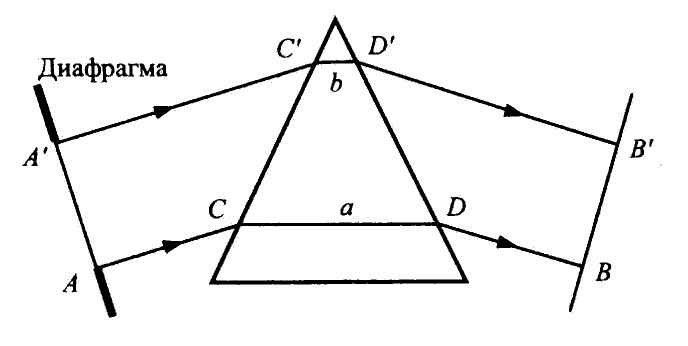
\includegraphics[width=0.4\textwidth]{figures/49_1.png}
    \caption{Призма, как спектральный прибор}
    \label{fig:pr}
\end{figure}
Начальное положение волнового $AA'$, а после $BB'$. Поскольку $BB'$ -- это участок волнового фронта, то данное направление можно рассматривать как направление на дифракционный максимум $m=0$ для $\lambda'$. 

По критерию Рэлея направление на дифракционный минимум $\lambda$ должен совпадать с максимумом $\lambda'$, тогда разность хода лучей $AB$ и $A' B'$ равна длине волны:
\begin{align*}
    &\text{max:} \ \ 
    &\left[AC + n(\lambda') a + DB\right] - \left[
        A'C' + n(\lambda') b + D' B'
    \right] = 0, \\
    &\text{min:} \ \ 
    &\left[AC + n(\lambda) a + DB\right] - 
    \left[
        A'C' + n(\lambda) b + D' B'
    \right] = \lambda,
\end{align*}
где $AA'$ и $BB'$ уже не представляют участков волнового фронта.  Вычитая два последних равенства, находим
\begin{equation*}
    \left[n(\lambda)-n(\lambda')\right]a - \left[n(\lambda)-n(\lambda')\right]b = \lambda,
\end{equation*}
что при рассмотрении близких $\lambda' - \lambda \ll\lambda$ и считая $\Delta \lambda = \lambda'-\lambda$ перейдёт в 
\begin{equation*}
    -(a-b) \frac{d n}{d \lambda} \Delta \lambda = \lambda,
    \hspace{0.5cm} \Rightarrow \hspace{0.5cm}
    R = \frac{\lambda}{\Delta \lambda} = - (a-b) \frac{d n}{d \lambda},
\end{equation*}
где $R > 0$ при $n'_\lambda < 0$ в области нормальной дисперсии.